\documentclass{beamer}
\usepackage{CJKutf8}
\usepackage{tikz}
\usetikzlibrary{calc}
\usepackage{clrscode3e}
\usepackage{ragged2e}


\setbeamertemplate{theorems}[numbered]
\newtheorem{Thm}{定理}[section]
\newtheorem*{Thm1}{定理6.3}
\theoremstyle{definition}
\newtheorem{Def}{定义}[section]
\theoremstyle{example}
\newtheorem*{Ex}{例:}


\begin{document}
\begin{CJK*}{UTF8}{gbsn}

\date{}
\author{陈建文}

\title{第六章 图的基本概念}
\begin{frame}
  \titlepage
\end{frame}
\section{图论的产生与发展史概述}
\begin{frame}
  \frametitle{6.1 图论的产生与发展史概述}
  \centering
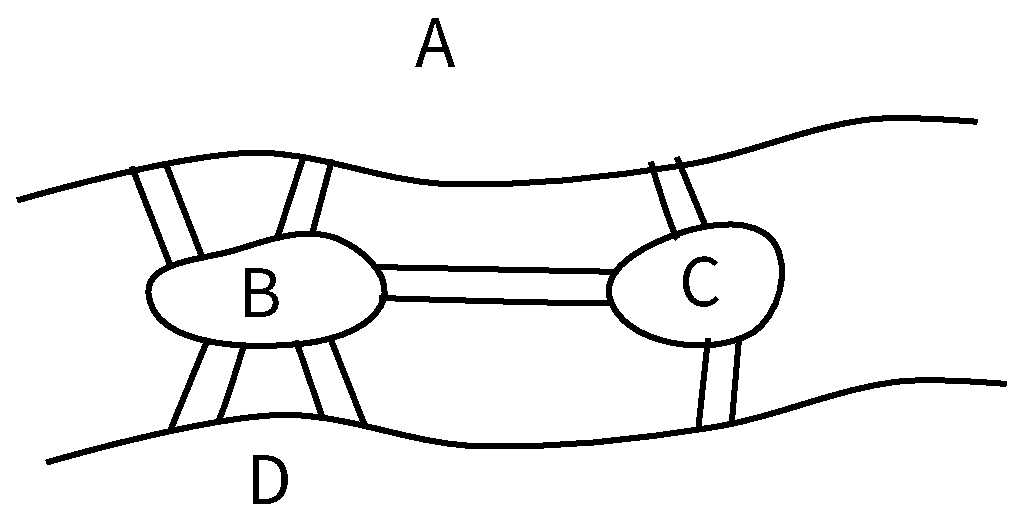
\includegraphics[width=5cm,height=4cm]{konigsberg} 
\end{frame}

\section{基本定义}
\begin{frame}
  \frametitle{6.2 基本定义}
设$V$为一个集合,$V$的一切二元子集之集合记为$\mathcal{P}_2(V)$,即
\begin{equation*}
  \mathcal{P}_2(V) = \{A|A \subseteq V \text{且} |A| = 2\}\text{。}
\end{equation*}
\begin{Def}\justifying\let\raggedright\justifying
  设$V$为一个非空有限集合,$E \subseteq \mathcal{P}_2(V)$,二元组$G = (V, E)$称为一个\alert{无向图}。$V$中的元素称为无向图$G$的\alert{顶点},$V$为\alert{顶点集};$E$中的元素称为无向图$G$的\alert{边},$E$为\alert{边集}。无向图简称\alert{图}。如果$|V|=p$,$|E|=q$,则称$G$为一个$(p,q)$图,即$G$是一个具有$p$个顶点$q$条边的图。
\end{Def}
      \centering
    \begin{tikzpicture}[auto,
    specification/.style ={circle, draw, thick, inner sep = 0pt, minimum size=2mm}]
   \node[specification] (A)  [label=0:$v_2$] at (18:1.3cm)  {};
   \node[specification] (B)  [label=90:$v_1$] at (90:1.3cm)  {};
   \node[specification] (C)  [label=180:$v_5$] at (162:1.3cm)  {};
   \node[specification] (D) [label=180:$v_4$] at (234:1.3cm)  {};
   \node[specification] (E)  [label=0:$v_3$] at (306:1.3cm)  {};      
   
   
   \draw[thick] (A) to  (B);
   \draw[thick] (B) to  (C);
   \draw[thick] (C) to  (D);
   \draw[thick] (D) to  (E);
   \draw[thick] (E) to  (A);
   \draw[thick] (A) to  (C);
   \draw[thick] (B) to  (E);
   \draw[thick] (C) to  (E);
   \draw[thick] (D) to  (A);
 \end{tikzpicture}
\end{frame}


\begin{frame}
  \frametitle{6.2 基本定义}
  \begin{Def}\justifying\let\raggedright\justifying
    在图$G=(V,E)$中,如果$\{u,v\}\in E$,则称\alert{顶点$u$与$v$邻接};若$x$与$y$是图$G$的两条边,并且仅有一个公共端点,即$|x \cap y|= 1$,则称\alert{边$x$与$y$邻接};如果$x=\{u,v\}$是图$G$的一条边,则称\alert{$u$与$x$互相关联},同样的,称\alert{$v$与$x$互相关联}。
  \end{Def}
        \centering
    \begin{tikzpicture}[auto,
    specification/.style ={circle, draw, thick, inner sep = 0pt, minimum size=2mm}]
   \node[specification] (A)  [label=0:$v_2$] at (18:1.3cm)  {};
   \node[specification] (B)  [label=90:$v_1$] at (90:1.3cm)  {};
   \node[specification] (C)  [label=180:$v_5$] at (162:1.3cm)  {};
   \node[specification] (D) [label=180:$v_4$] at (234:1.3cm)  {};
   \node[specification] (E)  [label=0:$v_3$] at (306:1.3cm)  {};      
   
   
   \draw[thick] (A) to  (B);
   \draw[thick] (B) to  (C);
   \draw[thick] (C) to  (D);
   \draw[thick] (D) to  (E);
   \draw[thick] (E) to  (A);
   \draw[thick] (A) to  (C);
   \draw[thick] (B) to  (E);
   \draw[thick] (C) to  (E);
   \draw[thick] (D) to  (A);
 \end{tikzpicture}

\end{frame}

\begin{frame}
  \frametitle{6.2 基本定义}
  \begin{Def}
   如果一个图中两个顶点间允许有多于一条边存在,则称为\alert{多重图},这些边称为\alert{多重边}; 如果一个图中允许联结一个顶点与其自身的边存在,则称为\alert{带环图},这些边称为\alert{环};允许有环或多重边存在的图,称之为\alert{伪图}。
  \end{Def}
\end{frame}


\begin{frame}
  \frametitle{6.2 基本定义}
  \begin{Def}
设$G=(V,E)$为一个图,如果$E=\Phi$,则称$G$为\alert{零图}; $(1,0)$图称为\alert{平凡图}。    
  \end{Def}
\end{frame}



\begin{frame}
  \frametitle{6.2 基本定义}
  \begin{Def}
    设$v$为图$G=(V,E)$的任意一个顶点,$G$中与$v$关联的边的数目称为顶点$v$的\alert{度},记为$\deg x$。
  \end{Def}
   \centering
    \begin{tikzpicture}[auto,
    specification/.style ={circle, draw, thick, inner sep = 0pt, minimum size=2mm}]
   \node[specification] (A)  [label=0:$v_2$] at (18:1.3cm)  {};
   \node[specification] (B)  [label=90:$v_1$] at (90:1.3cm)  {};
   \node[specification] (C)  [label=180:$v_5$] at (162:1.3cm)  {};
   \node[specification] (D) [label=180:$v_4$] at (234:1.3cm)  {};
   \node[specification] (E)  [label=0:$v_3$] at (306:1.3cm)  {};      
   
   
   \draw[thick] (A) to  (B);
   \draw[thick] (B) to  (C);
   \draw[thick] (C) to  (D);
   \draw[thick] (D) to  (E);
   \draw[thick] (E) to  (A);
   \draw[thick] (A) to  (C);
   \draw[thick] (B) to  (E);
   \draw[thick] (C) to  (E);
   \draw[thick] (D) to  (A);
 \end{tikzpicture}
\\  G   
\end{frame}

\begin{frame}
  \frametitle{6.2 基本定义}
  \begin{Thm}
    设$G=(V,E)$为一个具有$p$个顶点$q$条边的图,则$G$中各顶点度的和等于边的条数$q$的两倍,即
        \begin{equation*}
      \sum_{v \in V}\deg v = 2q
    \end{equation*}
  \end{Thm}
    \centering
    \begin{tikzpicture}[auto,
    specification/.style ={circle, draw, thick, inner sep = 0pt, minimum size=2mm}]
   \node[specification] (A)  [label=0:$v_2$] at (18:1.3cm)  {};
   \node[specification] (B)  [label=90:$v_1$] at (90:1.3cm)  {};
   \node[specification] (C)  [label=180:$v_5$] at (162:1.3cm)  {};
   \node[specification] (D) [label=180:$v_4$] at (234:1.3cm)  {};
   \node[specification] (E)  [label=0:$v_3$] at (306:1.3cm)  {};      
   
   
   \draw[thick] (A) to  (B);
   \draw[thick] (B) to  (C);
   \draw[thick] (C) to  (D);
   \draw[thick] (D) to  (E);
   \draw[thick] (E) to  (A);
   \draw[thick] (A) to  (C);
   \draw[thick] (B) to  (E);
   \draw[thick] (C) to  (E);
   \draw[thick] (D) to  (A);
 \end{tikzpicture}
 \\  G   
\end{frame}


\begin{frame}
  \frametitle{6.2 基本定义}
  \begin{Thm}
       在任一图中,度为奇数的顶点的数目必为偶数。
  \end{Thm}
\centering
    \begin{tikzpicture}[auto,
    specification/.style ={circle, draw, thick, inner sep = 0pt, minimum size=2mm}]
   \node[specification] (A)  [label=0:$v_2$] at (18:1.3cm)  {};
   \node[specification] (B)  [label=90:$v_1$] at (90:1.3cm)  {};
   \node[specification] (C)  [label=180:$v_5$] at (162:1.3cm)  {};
   \node[specification] (D) [label=180:$v_4$] at (234:1.3cm)  {};
   \node[specification] (E)  [label=0:$v_3$] at (306:1.3cm)  {};      
   
   
   \draw[thick] (A) to  (B);
   \draw[thick] (B) to  (C);
   \draw[thick] (C) to  (D);
   \draw[thick] (D) to  (E);
   \draw[thick] (E) to  (A);
   \draw[thick] (A) to  (C);
   \draw[thick] (B) to  (E);
   \draw[thick] (C) to  (E);
   \draw[thick] (D) to  (A);
 \end{tikzpicture}
\\  G 
\end{frame}
\begin{frame}
  \frametitle{6.2 基本定义}
  \begin{Def}
    图$G$称为\alert{$r$度正则图},如果$G$的每个顶点的度都等于$r$。3度正则图也叫三次图。
    一个具有$p$个顶点的$p-1$度正则图称为包含$p$个顶点的\alert{完全图},记为$K_p$。
  \end{Def}
\end{frame}
\begin{frame}
  \frametitle{6.2 基本定义}
    \begin{minipage}[c]{0.4\textwidth}
\centering
    \begin{tikzpicture}[auto,
    specification/.style ={circle, draw, thick, inner sep = 0pt, minimum size=2mm}]
   \node[specification] (A)  [label=0:$v_2$] at (18:1.3cm)  {};
   \node[specification] (B)  [label=90:$v_1$] at (90:1.3cm)  {};
   \node[specification] (C)  [label=180:$v_5$] at (162:1.3cm)  {};
   \node[specification] (D) [label=180:$v_4$] at (234:1.3cm)  {};
   \node[specification] (E)  [label=0:$v_3$] at (306:1.3cm)  {};      
   
   
   \draw[thick] (A) to  (B);
   \draw[thick] (B) to  (C);
   \draw[thick] (C) to  (D);
   \draw[thick] (D) to  (E);
   \draw[thick] (E) to  (A);
   \draw[thick] (A) to  (C);
   \draw[thick] (B) to  (E);
   \draw[thick] (C) to  (E);
   \draw[thick] (D) to  (A);
 \end{tikzpicture}
\\ \centering G 
    \end{minipage}\hspace{2cm}
    \begin{minipage}[c]{0.4\textwidth}
\centering
    \begin{tikzpicture}[auto,
    specification/.style ={circle, draw, thick, inner sep = 0pt, minimum size=2mm}]
   \node[specification] (A)  [label=0:$v_2$] at (18:1.3cm)  {};
   \node[specification] (B)  [label=90:$v_1$] at (90:1.3cm)  {};
   \node[specification] (E)  [label=0:$v_3$] at (306:1.3cm)  {};      
   
   
   \draw[thick] (A) to  (B);
   \draw[thick] (B) to  (E);
 \end{tikzpicture}
\\ \centering H 
    \end{minipage}
    \pause
  \begin{Def}
    设$G=(V,E)$为一个图,图$H=(V_1,E_1)$称为$G$的一个子图,当且仅当$V_1$为$V$的
    非空子集且$E_1$为$E$的子集。如果$H \neq G$,则称$H$为$G$的\alert{真子图}。
  \end{Def}
\end{frame}

\begin{frame}
  \frametitle{6.2 基本定义}
  \begin{minipage}[c]{0.4\textwidth}
    \centering
    \begin{tikzpicture}[auto,
    specification/.style ={circle, draw, thick, inner sep = 0pt, minimum size=2mm}]
   \node[specification] (A)  [label=0:$v_2$] at (18:1.3cm)  {};
   \node[specification] (B)  [label=90:$v_1$] at (90:1.3cm)  {};
   \node[specification] (C)  [label=180:$v_5$] at (162:1.3cm)  {};
   \node[specification] (D) [label=180:$v_4$] at (234:1.3cm)  {};
   \node[specification] (E)  [label=0:$v_3$] at (306:1.3cm)  {};      
   
   
   \draw[thick] (A) to  (B);
   \draw[thick] (B) to  (C);
   \draw[thick] (C) to  (D);
   \draw[thick] (D) to  (E);
   \draw[thick] (E) to  (A);
   \draw[thick] (A) to  (C);
   \draw[thick] (B) to  (E);
   \draw[thick] (C) to  (E);
   \draw[thick] (D) to  (A);
 \end{tikzpicture}
\\ \centering G 
    \end{minipage}\hspace{2cm}
    \begin{minipage}[c]{0.4\textwidth}
\centering
    \begin{tikzpicture}[auto,
    specification/.style ={circle, draw, thick, inner sep = 0pt, minimum size=2mm}]
   \node[specification] (A)  [label=0:$v_2$] at (18:1.3cm)  {};
   \node[specification] (B)  [label=90:$v_1$] at (90:1.3cm)  {};
   \node[specification] (C)  [label=180:$v_5$] at (162:1.3cm)  {};
   \node[specification] (D) [label=180:$v_4$] at (234:1.3cm)  {};
   \node[specification] (E)  [label=0:$v_3$] at (306:1.3cm)  {};      
   
   
   \draw[thick] (A) to  (B);
   \draw[thick] (B) to  (E);
 \end{tikzpicture}
 \\ \centering H 
    \end{minipage}
    \pause
  \begin{Def}
    设$G=(V,E)$为一个图,如果$F\subseteq E$,则称$G$的子图$H=(V,F)$ 为$G$的一个\alert{生成子图}。
  \end{Def}
\end{frame}

\begin{frame}
  \frametitle{6.2 基本定义}
    \begin{minipage}[c]{0.4\textwidth}
    \centering
    \begin{tikzpicture}[auto,
    specification/.style ={circle, draw, thick, inner sep = 0pt, minimum size=2mm}]
   \node[specification] (A)  [label=0:$v_2$] at (18:1.3cm)  {};
   \node[specification] (B)  [label=90:$v_1$] at (90:1.3cm)  {};
   \node[specification] (C)  [label=180:$v_5$] at (162:1.3cm)  {};
   \node[specification] (D) [label=180:$v_4$] at (234:1.3cm)  {};
   \node[specification] (E)  [label=0:$v_3$] at (306:1.3cm)  {};      
   
   
   \draw[thick] (A) to  (B);
   \draw[thick] (B) to  (C);
   \draw[thick] (C) to  (D);
   \draw[thick] (D) to  (E);
   \draw[thick] (E) to  (A);
   \draw[thick] (A) to  (C);
   \draw[thick] (B) to  (E);
   \draw[thick] (C) to  (E);
   \draw[thick] (D) to  (A);
 \end{tikzpicture}
 \\ \centering G 
    \end{minipage}\hspace{2cm}
    \begin{minipage}[c]{0.4\textwidth}
    \centering
    \begin{tikzpicture}[auto,
    specification/.style ={circle, draw, thick, inner sep = 0pt, minimum size=2mm}]
   \node[specification] (A)  [label=0:$v_2$] at (18:1.3cm)  {};
   \node[specification] (B)  [label=90:$v_1$] at (90:1.3cm)  {};
   \node[specification] (E)  [label=0:$v_3$] at (306:1.3cm)  {};      
   
   
   \draw[thick] (A) to  (B);
   \draw[thick] (E) to  (A);
   \draw[thick] (B) to  (E);
 \end{tikzpicture}
\\ \centering H 
    \end{minipage}

    \pause
  \begin{Def}
    设$G$的子图$H$具有某种性质,若$G$中不存在与$H$不同的具有此性质且包含$H$的子图,则称$H$是具有此性质的\alert{极大子图}。
  \end{Def}
\pause
  \begin{Def}
    设$S$为图$G=(V,E)$的顶点集$V$的非空子集,则$G$的以$S$为顶点集的极大子图称为由$S$导出的子图,记为$\langle S \rangle$。
形式的,
\begin{equation*}
  \langle S \rangle=(S, \mathcal{P}_2(S) \cap E)
\end{equation*}
  \end{Def}
\end{frame}
\begin{frame}
  \frametitle{6.2 基本定义}
    \begin{minipage}[c]{0.4\textwidth}
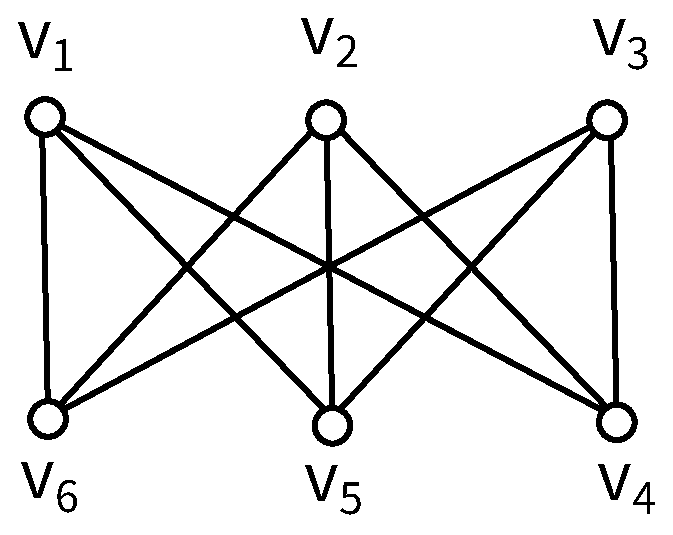
\includegraphics[width=4cm,height=3cm]{k33} \\ \centering G 
    \end{minipage}\hspace{2cm}
    \begin{minipage}[c]{0.4\textwidth}
\includegraphics[width=4cm,height=3cm]{isomorphic} \\ \centering H 
    \end{minipage}
    \pause
  \begin{Def}
    设$G=(V,E)$, $H = (U, F)$为两个图,如果存在一个一一对应$\phi:V \to
    U$,使得$\{u,v\} \in E$当且仅当$\{\phi(u),\phi(v)\} \in F$,则称$G$与$H$\alert{同构}。
  \end{Def}
\end{frame}
\section{路、圈、连通图
}
\begin{frame}
  \frametitle{6.3 路、圈、连通图}
  \begin{Def}
    设$G=(V,E)$为一个图。$G$的一条\alert{通道}是$G$的顶点和边的一个交错序列
    \[v_0,x_1,v_1,x_2,v_2,x_3,\ldots,v_{n-1},x_n,v_n\]
    其中$x_i=v_{i-1}v_i,i=1,2,\ldots,n$。$n$称为通道的长。这样的通道常称为$v_0-v_n$通道,并简记为$v_0v_1v_2\ldots   v_n$。当$v_0=v_n$时,则称此通道为\alert{闭通道}。
  \end{Def}
  \centering
  \begin{tikzpicture}[auto,
    specification/.style ={circle, draw, thick}]
   \node[specification] (E) [label=-135:$v_5$] at (0,0)  {};
   \node[specification] (F) [label=135:$v_3$] at (0,2)  {};
   \node[specification] (G) [label=45:$v_2$] at (2,2)  {};
   \node[specification] (H) [label=-45:$v_4$] at (2,0)  {};
   \node[specification] (I) [label=-45:$v_1$] at (4,2)  {};
   
   \draw[thick] (E) to  (F);
   \draw[thick] (F) to  (G);
   \draw[thick] (G) to  (H);
   \draw[thick] (H) to  (E);
   \draw[thick] (E) to  (G);
   \draw[thick] (G) to  (I);
 \end{tikzpicture}  
 \\  G   
\end{frame}

\begin{frame}
  \frametitle{6.3 路、圈、连通图}
  \begin{Def}
   如果图中一条通道上的各边互不相同,则称此通道为图的\alert{迹}。如果一条闭通道上的各边互不相同,则此闭通道称为\alert{闭迹}。
  \end{Def}
  \centering
  \begin{tikzpicture}[auto,
    specification/.style ={circle, draw, thick}]
   \node[specification] (E) [label=-135:$v_5$] at (0,0)  {};
   \node[specification] (F) [label=135:$v_3$] at (0,2)  {};
   \node[specification] (G) [label=45:$v_2$] at (2,2)  {};
   \node[specification] (H) [label=-45:$v_4$] at (2,0)  {};
   \node[specification] (I) [label=-45:$v_1$] at (4,2)  {};
   
   \draw[thick] (E) to  (F);
   \draw[thick] (F) to  (G);
   \draw[thick] (G) to  (H);
   \draw[thick] (H) to  (E);
   \draw[thick] (E) to  (G);
   \draw[thick] (G) to  (I);
 \end{tikzpicture}  
 \\  G   
\end{frame}

\begin{frame}
  \frametitle{6.3 路、圈、连通图}
  \begin{Def}
    如果一条通道上的各顶点互不相同,则称此通道为\alert{路}。如果闭通道上各顶点互不相同,则称此闭通道为\alert{圈},或\alert{回路}。
  \end{Def}
  \centering
  \begin{tikzpicture}[auto,
    specification/.style ={circle, draw, thick}]
   \node[specification] (E) [label=-135:$v_5$] at (0,0)  {};
   \node[specification] (F) [label=135:$v_3$] at (0,2)  {};
   \node[specification] (G) [label=45:$v_2$] at (2,2)  {};
   \node[specification] (H) [label=-45:$v_4$] at (2,0)  {};
   \node[specification] (I) [label=-45:$v_1$] at (4,2)  {};
   
   \draw[thick] (E) to  (F);
   \draw[thick] (F) to  (G);
   \draw[thick] (G) to  (H);
   \draw[thick] (H) to  (E);
   \draw[thick] (E) to  (G);
   \draw[thick] (G) to  (I);
 \end{tikzpicture}  
 \\  G   
\end{frame}

\begin{frame}
  \frametitle{6.3 路、圈、连通图}
  \begin{Def}
   设$G=(V,E)$为一个图,如果$G$中任两个不同顶点间至少有一条路联结,则称$G$为一个\alert{连通图}。
  \end{Def}
    \centering
    \begin{tikzpicture}[auto,
    specification/.style ={circle, draw, thick, inner sep = 0pt, minimum size=2mm}]
   \node[specification] (A)  [label=0:$v_2$] at (18:1.3cm)  {};
   \node[specification] (B)  [label=90:$v_1$] at (90:1.3cm)  {};
   \node[specification] (C)  [label=180:$v_5$] at (162:1.3cm)  {};
   \node[specification] (D) [label=180:$v_4$] at (234:1.3cm)  {};
   \node[specification] (E)  [label=0:$v_3$] at (306:1.3cm)  {};      
   
   
   \draw[thick] (A) to  (B);
   \draw[thick] (B) to  (C);
   \draw[thick] (C) to  (D);
   \draw[thick] (D) to  (E);
   \draw[thick] (E) to  (A);
   \draw[thick] (A) to  (C);
   \draw[thick] (B) to  (E);
   \draw[thick] (C) to  (E);
   \draw[thick] (D) to  (A);
 \end{tikzpicture}
 \\  G   
\end{frame}

\begin{frame}
  \frametitle{6.3 路、圈、连通图}
  \centering
  \begin{minipage}{0.33\linewidth}
    \centering
    \begin{tikzpicture}[auto,
    specification/.style ={circle, draw, thick}]
   \node[specification] (A) [label=-135:$v_1$] at (0,0)  {};
   \node[specification] (B) [label=135:$v_2$] at (0,2)  {};
   \node[specification] (C) [label=45:$v_3$] at (2,2)  {};
   \node[specification] (D) [label=-45:$v_4$] at (2,0)  {};
   \draw[thick] (A) to  (B);
   \draw[thick] (B) to  (C);
   \draw[thick] (C) to  (D);
   \draw[thick] (D) to  (A);
 \end{tikzpicture}
\end{minipage}\hfill
\begin{minipage}{0.33\linewidth}
  \centering
  \begin{tikzpicture}[auto,
    specification/.style ={circle, draw, thick}]
   \node[specification] (E) [label=-135:$v_5$] at (0,0)  {};
   \node[specification] (F) [label=135:$v_6$] at (0,2)  {};
   \node[specification] (G) [label=45:$v_7$] at (2,2)  {};
   \node[specification] (H) [label=-45:$v_8$] at (2,0)  {};
   \draw[thick] (E) to  (F);
   \draw[thick] (F) to  (G);
   \draw[thick] (G) to  (H);
   \draw[thick] (H) to  (E);
   \draw[thick] (E) to  (G);
 \end{tikzpicture}  
\end{minipage}\hfill
\begin{minipage}{0.33\linewidth}
  \centering
  \begin{tikzpicture}[auto,
    specification/.style ={circle, draw, thick}]
   \node[specification] (I) [label=-135:$v_9$] at (0,0)  {};
   \node[specification] (J) [label=135:$v_{10}$] at (1,2)  {};
   \node[specification] (K) [label=-45:$v_{11}$] at (2,0)  {};
   \draw[thick] (I) to  (J);
   \draw[thick] (J) to  (K);
 \end{tikzpicture}
\end{minipage}
\vspace*{2cm}
$G$
\end{frame}

\begin{frame}
  \frametitle{6.3 路、圈、连通图}
  \begin{minipage}{0.33\linewidth}
    \centering
    \begin{tikzpicture}[auto,
    specification/.style ={circle, draw, thick}]
   \node[specification] (A) [label=-135:$v_1$] at (0,0)  {};
   \node[specification] (B) [label=135:$v_2$] at (0,2)  {};
   \node[specification] (C) [label=45:$v_3$] at (2,2)  {};
   \node[specification] (D) [label=-45:$v_4$] at (2,0)  {};
   \draw[thick] (A) to  (B);
   \draw[thick] (B) to  (C);
   \draw[thick] (C) to  (D);
   \draw[thick] (D) to  (A);
 \end{tikzpicture}\\
 $G_1$
\end{minipage}\hfill
\begin{minipage}{0.33\linewidth}
  \centering
  \begin{tikzpicture}[auto,
    specification/.style ={circle, draw, thick}]
   \node[specification] (E) [label=-135:$v_5$] at (0,0)  {};
   \node[specification] (F) [label=135:$v_6$] at (0,2)  {};
   \node[specification] (G) [label=45:$v_7$] at (2,2)  {};
   \node[specification] (H) [label=-45:$v_8$] at (2,0)  {};
   \draw[thick] (E) to  (F);
   \draw[thick] (F) to  (G);
   \draw[thick] (G) to  (H);
   \draw[thick] (H) to  (E);
   \draw[thick] (E) to  (G);
 \end{tikzpicture}  \\
 $G_2$
\end{minipage}\hfill
\begin{minipage}{0.33\linewidth}
  \centering
  \begin{tikzpicture}[auto,
    specification/.style ={circle, draw, thick}]
   \node[specification] (I) [label=-135:$v_9$] at (0,0)  {};
   \node[specification] (J) [label=135:$v_{10}$] at (1,2)  {};
   \node[specification] (K) [label=-45:$v_{11}$] at (2,0)  {};
   \draw[thick] (I) to  (J);
   \draw[thick] (J) to  (K);
 \end{tikzpicture}\\
 $G_3$
\end{minipage}
\end{frame}

\begin{frame}
  \frametitle{6.3 路、圈、连通图}
  \begin{Def}
    图$G$的极大连通子图称为$G$的一个\alert{支}。
  \end{Def}
  \begin{minipage}{0.33\linewidth}
    \centering
    \begin{tikzpicture}[auto,
    specification/.style ={circle, draw, thick}]
   \node[specification] (A) [label=-135:$v_1$] at (0,0)  {};
   \node[specification] (B) [label=135:$v_2$] at (0,2)  {};
   \node[specification] (C) [label=45:$v_3$] at (2,2)  {};
   \node[specification] (D) [label=-45:$v_4$] at (2,0)  {};
   \draw[thick] (A) to  (B);
   \draw[thick] (B) to  (C);
   \draw[thick] (C) to  (D);
   \draw[thick] (D) to  (A);
 \end{tikzpicture}\\
 $G_1$
\end{minipage}\hfill
\begin{minipage}{0.33\linewidth}
  \centering
  \begin{tikzpicture}[auto,
    specification/.style ={circle, draw, thick}]
   \node[specification] (E) [label=-135:$v_5$] at (0,0)  {};
   \node[specification] (F) [label=135:$v_6$] at (0,2)  {};
   \node[specification] (G) [label=45:$v_7$] at (2,2)  {};
   \node[specification] (H) [label=-45:$v_8$] at (2,0)  {};
   \draw[thick] (E) to  (F);
   \draw[thick] (F) to  (G);
   \draw[thick] (G) to  (H);
   \draw[thick] (H) to  (E);
   \draw[thick] (E) to  (G);
 \end{tikzpicture}  \\
 $G_2$
\end{minipage}\hfill
\begin{minipage}{0.33\linewidth}
  \centering
  \begin{tikzpicture}[auto,
    specification/.style ={circle, draw, thick}]
   \node[specification] (I) [label=-135:$v_9$] at (0,0)  {};
   \node[specification] (J) [label=135:$v_{10}$] at (1,2)  {};
   \node[specification] (K) [label=-45:$v_{11}$] at (2,0)  {};
   \draw[thick] (I) to  (J);
   \draw[thick] (J) to  (K);
 \end{tikzpicture}\\
 $G_3$
\end{minipage}
\end{frame}

\begin{frame}
  \frametitle{6.3 路、圈、连通图}
  \begin{Thm}
    设$G=(V,E)$是一个图。在$V$上定义二元关系$\cong$如下:\[\forall u, v \in V, u
      \cong v\text{当且仅当}u\text{与}v\text{间有一条路,}\]则$\cong$为$V$上的等价关系,$G$的支就是关于$\cong$的每个等价类的导出子图。
  \end{Thm}
\end{frame}


\section{补图、偶图}
\begin{frame}
  \frametitle{6.4 补图、偶图}
  \begin{Def}
    设$G=(V,E)$是一个图,图$G^c=(V, \mathcal{P}_2(V)\setminus E)$称为$G$的\alert{补图}。如果$G$与$G^c$同构,则称$G$是\alert{自补图}。
  \end{Def}
  \begin{minipage}{0.49\linewidth}
    \centering
    \begin{tikzpicture}[auto,
    specification/.style ={circle, draw, thick}]
   \node[specification] (A) [label=-135:A] at (0,0)  {};
   \node[specification] (B) [label=135:B] at (0,2)  {};
   \node[specification] (C) [label=45:C] at (2,2)  {};
   \node[specification] (D) [label=-45:D] at (2,0)  {};
   \draw[thick] (A) to  (B);
   \draw[thick] (A) to  (C);
   \draw[thick] (A) to  (D);
 \end{tikzpicture}\\
 $G$
\end{minipage}\pause
  \begin{minipage}{0.49\linewidth}
    \centering
    \begin{tikzpicture}[auto,
    specification/.style ={circle, draw, thick}]
   \node[specification] (A) [label=-135:A] at (0,0)  {};
   \node[specification] (B) [label=135:B] at (0,2)  {};
   \node[specification] (C) [label=45:C] at (2,2)  {};
   \node[specification] (D) [label=-45:D] at (2,0)  {};
   \draw[thick] (B) to  (C);
   \draw[thick] (C) to  (D);
   \draw[thick] (D) to  (B);
 \end{tikzpicture}\\
 $G^c$
\end{minipage}        

\end{frame}

\begin{frame}
  \frametitle{6.4 补图、偶图}
  \begin{Def}
    设$G=(V,E)$是一个图,图$G^c=(V, \mathcal{P}_2(V)\setminus E)$称为$G$的\alert{补图}。如果$G$与$G^c$同构,则称$G$是\alert{自补图}。
  \end{Def}
  \begin{minipage}{0.49\linewidth}
    \centering
    \begin{tikzpicture}[auto,
    specification/.style ={circle, draw, thick}]
   \node[specification] (A) [label=-135:A] at (0,0)  {};
   \node[specification] (B) [label=135:B] at (0,2)  {};
   \node[specification] (C) [label=45:C] at (2,2)  {};
   \node[specification] (D) [label=-45:D] at (2,0)  {};
   \draw[thick] (A) to  (B);
   \draw[thick] (B) to  (C);
   \draw[thick] (C) to  (D);
 \end{tikzpicture}\\
 $G$
\end{minipage}\pause
  \begin{minipage}{0.49\linewidth}
    \centering
    \begin{tikzpicture}[auto,
    specification/.style ={circle, draw, thick}]
   \node[specification] (A) [label=-135:A] at (0,0)  {};
   \node[specification] (B) [label=135:B] at (0,2)  {};
   \node[specification] (C) [label=45:C] at (2,2)  {};
   \node[specification] (D) [label=-45:D] at (2,0)  {};
   \draw[thick] (A) to  (D);
   \draw[thick] (B) to  (D);
   \draw[thick] (A) to  (C);
 \end{tikzpicture}\\
 $G^c$
\end{minipage}        
\end{frame}

\begin{frame}
  \frametitle{6.4 补图、偶图}
  \begin{Thm}
    对任一有$6$个顶点的图$G$,$G$中或$G^c$中有一个三角形。
  \end{Thm}
  \begin{proof}[证明]
    设图$G$的顶点集为$V=\{v_1,v_2,v_3,v_4,v_5,v_6\}$,考虑顶点$v_1$。
    \begin{itemize}
    \item 存在三个顶点,其中的每个顶点都与顶点$v_1$相邻接。不失一般性,不妨设这
      个三个顶点为$v_2,v_3,v_4$。
      \begin{itemize}
      \item[-] 在顶点$v_2,v_3,v_4$中,存在两个顶点相邻接。
      \item[-] 在顶点$v_2,v_3,v_4$中,任意两个顶点都不邻接。
      \end{itemize}
    \item 存在三个顶点,其中的每个顶点都与顶点$v_1$不邻接。不失一般性,不妨设这
      个三个顶点为$v_2,v_3,v_4$。
      \begin{itemize}
      \item[-] 在顶点$v_2,v_3,v_4$中,存在两个顶点不邻接。
      \item[-] 在顶点$v_2,v_3,v_4$中,任意两个顶点互相邻接。
      \end{itemize}

    \end{itemize}
  \end{proof}
\end{frame}

\begin{frame}
  \frametitle{6.4 补图、偶图}
  \begin{Def}
    对任意的正整数$m$,$n$,$m \geq 2$,$n \geq 2$,求一个最小的正整数$r(m,n)$,
    使得任何有$r(m,n)$个顶点的图$G$中一定含有一个$K_m$或者图$G^c$中一定含有一个$K_n$,这里的数$r(m,n)$称为\alert{拉姆齐数}。
  \end{Def}
\end{frame}

\begin{frame}
  \frametitle{6.4 补图、偶图}
  \begin{Def}\justifying\let\raggedright\justifying
    设$G=(V,E)$为一个图,如果$G$的顶点集$V$有一个二划分$\{V_1,V_2\}$,
    使得$G$的任一条边的两个端点一个在$V_1$中,另一个在$V_2$中,则称$G$为\alert{偶图}。如果$\forall u \in V_1, v \in V_2$均有$uv \in E$,则称$G$为\alert{完全偶图},记为$K_{m,n}$,其中$|V_1|=m,|V_2|=n$。
  \end{Def}
\end{frame}

\begin{frame}
  \frametitle{6.4 补图、偶图}
  \begin{Def}
    设$G=(V,E)$是一个图,$u$和$v$是$G$的顶点。联结$u$和$v$的最短路的长称为$u$与$v$之间的\alert{距离},并记为$d(u,v)$。如果$u$与$v$间在$G$中没有路,则定义$d(u,v)=\infty$。
  \end{Def}
\end{frame}

\begin{frame}
  \frametitle{6.4 补图、偶图}
  \begin{Thm}
    图$G$为偶图的充分必要条件是它的所有圈都是偶数长。
  \end{Thm}
\end{frame}

\begin{frame}
  \frametitle{6.4 补图、偶图}
  \begin{Thm}
    所有具有$p$个顶点而没有三角形的图中最多有$\llcorner p^2/4\lrcorner$条边。
  \end{Thm}
\end{frame}

% \begin{frame}
%   \frametitle{匹配}
%   \begin{definition6.4.4}
%     设$G=(V,E)$是一个图,$G$的任两条不邻接的边$x$与$y$称为互相\alert{独
%       立}的。$G$的边集$E$的子集$Y$称为$G$的一个\alert{匹配},如果$Y$中任意两条边都是互相独立的。
%   \end{definition6.4.4}
% \pause
% \centering
% 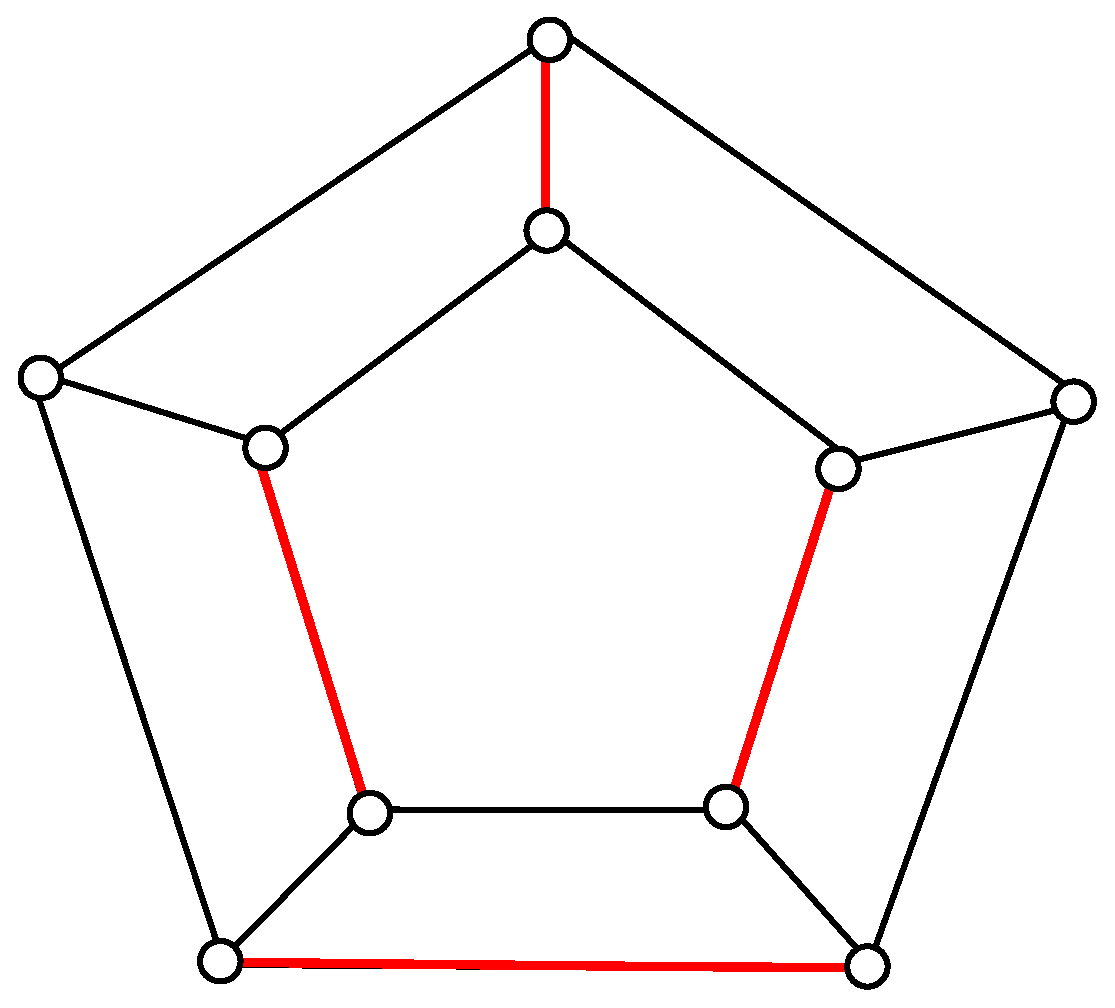
\includegraphics[width=5cm,height=4cm]{matching}
% \end{frame}
% \begin{frame}
%   \frametitle{匹配}
%   \begin{definition6.4.5}
%     设$Y$是图$G=(V,E)$的一个匹配,如果$2|Y|=|V|$,则称$Y$为$G$的一个\alert{完美匹配}。
%   \end{definition6.4.5}
% \pause
% \centering
% 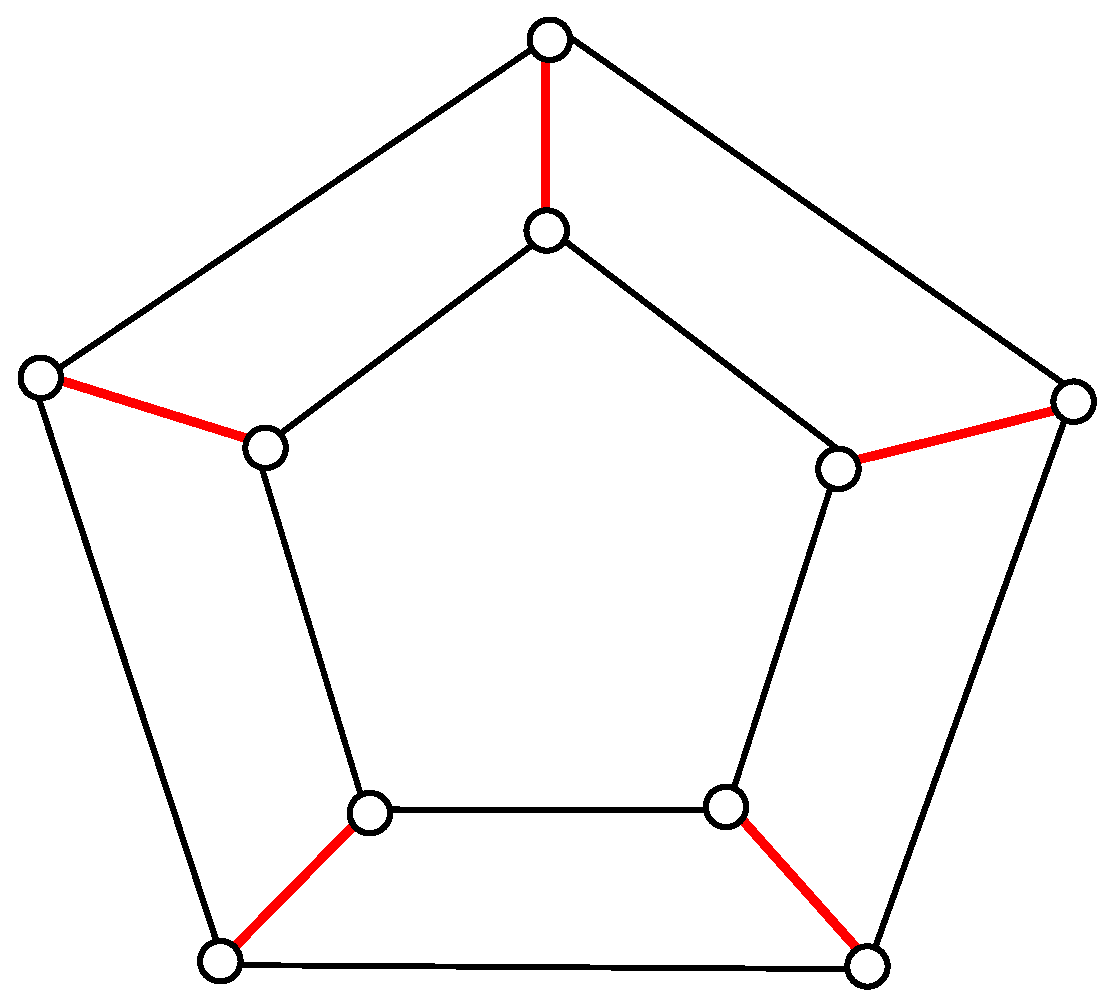
\includegraphics[width=5cm,height=4cm]{perfect}
% \end{frame}

% \begin{frame}
%   \frametitle{匹配}
%     \begin{definition6.4.6}
%    设$Y$是图$G=(V,E)$的一个匹配,如果对于$G$的任一匹配$Y'$,恒有$|Y'|\leq |Y|$, 则称$Y$为$G$的一个\alert{最大匹配}。
%   \end{definition6.4.6}
% \pause
% \centering
% 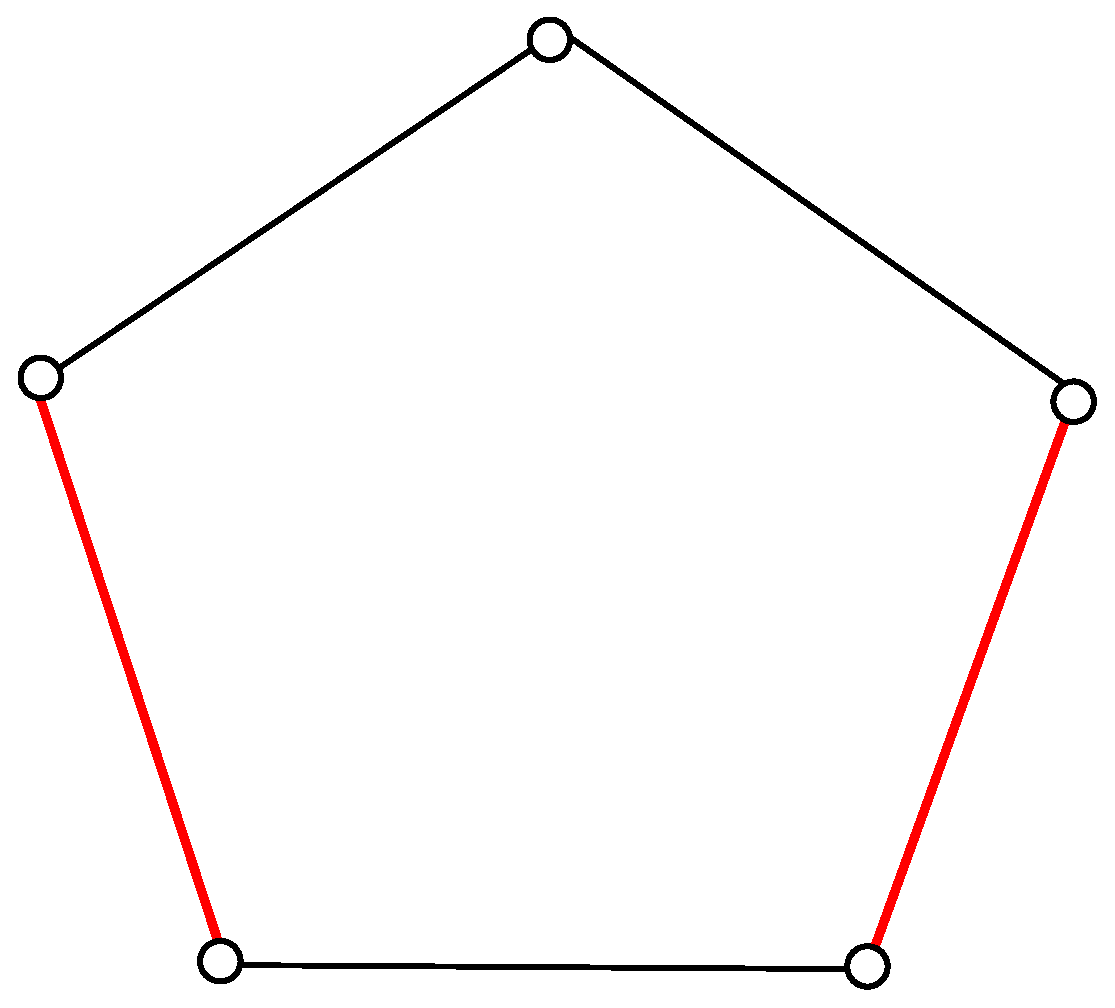
\includegraphics[width=4cm,height=3cm]{maximum}
% \end{frame}
% \begin{frame}
%   \frametitle{匹配}
%   \begin{definition6.4.7}
%     设$G=((V_1,V_2),E)$是一个偶图,如果存在$G$的一
%     个匹配$Y$使得$|Y|=min\{|V_1|,|V_2|\}$,则称$Y$是偶图$G$的一个\alert{完全匹配}。
%   \end{definition6.4.7}
% \end{frame}

%   \begin{frame}
%     \frametitle{Stable Matching}
%     \begin{definition1}
%       A certain community consists of $n$ men and $n$ women. Each person ranks those of the opposite sex in accordance with his or her preferences for a marriage partner. We seek a satisfactory way of marrying off all members of the community. We call a set of marriages unstable if under it there are a man and a woman who are not married to each other but prefer each other to their actual mates. For any pattern of preferences is it possible to find a stable set of marriages?
%     \end{definition1}
%   \end{frame}
  
%   \begin{frame}
%     \frametitle{Stable Matching}
%       \begin{codebox}
%     \Procname{$\proc{Gale-Shapley}(manPref,womanPref)$}
%     \zi Initially all $m \in M$ and $w \in W$ are free
%     \zi \While there is a man $m$ who is free
%     \zi \Do
%            Choose such a man $m$
%     \zi       $w \gets $ the highest-ranked woman in m's preference list \\   $\quad\quad\quad$to whom m has not yet proposed
%     \zi \If $w$ is free then
%     \zi \Then $(m,w)$ become engaged
%     \zi \Else
%     \zi $w$ is currently engaged to $m'$
%     \zi \If $w$ prefers $m'$ to $m$ 
%     \zi \Then $m$ remains free
%     \zi \Else
%     \zi $(m,w)$ become engaged
%     \zi $m'$ becomes free
%     \End
%      \End
%     \End
%     \zi \Return S 
%   \end{codebox}
% \end{frame}
% \begin{frame}
%   \frametitle{Stable Matching}
%   \begin{Thm1}
%     The G-S algorithm terminates.
%   \end{Thm1}
% \end{frame}

% \begin{frame}
%   \frametitle{Stable Matching}
%   \begin{Thm2}
%     The G-S algorithm returns a stable matching.
%   \end{Thm2}
% \end{frame}

% \begin{frame}
%   \frametitle{Stable Matching}
%   \begin{Thm3}
%     In the stable matching returned from the G-S algorithm, each man is paired with his best valid partner.
%   \end{Thm3}
% \end{frame}

% \begin{frame}
%   \frametitle{Stable Matching}
%   \begin{Thm4}
%     In the stable matching returned from the G-S algorithm, each woman is paired with her worst valid partner.
%   \end{Thm4}
% \end{frame}

\section{欧拉图}
\begin{frame}
  \frametitle{6.5 欧拉图}
\centering
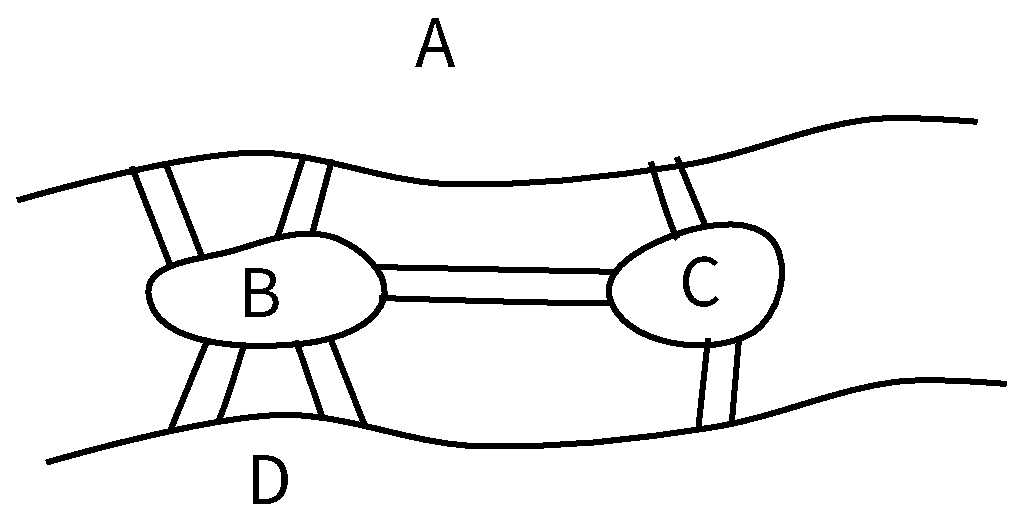
\includegraphics[width=5cm,height=4cm]{konigsberg} 
    \pause
  \begin{Def}
    包含图的所有顶点和所有边的闭迹称为\alert{欧拉闭迹}。存在一条欧拉闭迹的图称为\alert{欧拉图}。
  \end{Def}

\end{frame}


\begin{frame}
  \frametitle{6.5 欧拉图}
  \begin{Thm}
    图G是欧拉图当且仅当$G$是连通的且每个顶点的度是偶数。
  \end{Thm}

\end{frame}

\begin{frame}
  \frametitle{6.5 欧拉图}
  \begin{Def}
    包含图的所有顶点和边的迹称为\alert{欧拉迹}。
  \end{Def}

\end{frame}

\begin{frame}
  \frametitle{6.5 欧拉图}
  \begin{Thm}
    图G有一条欧拉开迹当且仅当$G$是连通的且恰有两个奇度顶点。
  \end{Thm}

\end{frame}


\begin{frame}
  \frametitle{6.5 欧拉图}
  \begin{Thm}
    设$G$是连通图,$G$恰有$2n$个奇度顶点,$n \geq 1$,则$G$的全部边可以排成$n$条
    开迹,且不能排成少于$n$条开迹。  \end{Thm}

\end{frame}

% \begin{frame}
%   \frametitle{6.6 哈密顿图}
% \centering
% 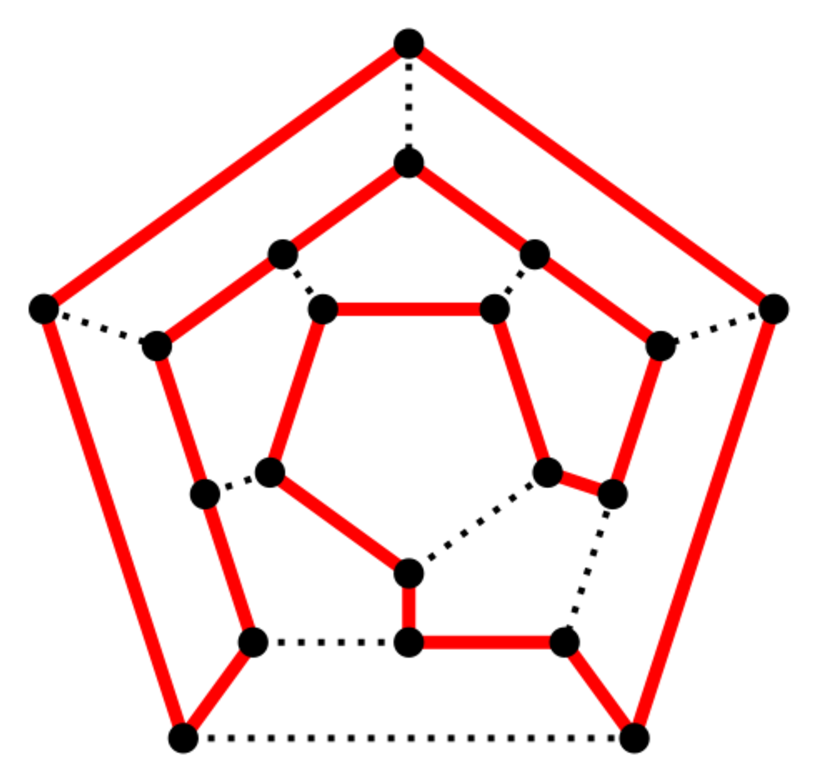
\includegraphics[width=5cm,height=4cm]{hamiltonian} 
%  \pause
%   \begin{definition6.6.1}
%     图$G$的一条包含所有顶点的路称为$G$的一条\alert{哈密顿路};图$G$的一个包含所有顶点的圈称为$G$的一个\alert{哈密顿圈}。具有哈密顿圈的图称为\alert{哈密顿图}。
%   \end{definition6.6.1}
% \end{frame}
\section{哈密顿图}
\begin{frame}
  \frametitle{6.6 哈密顿图}
  \centering
    \begin{tikzpicture}[auto,
    specification/.style ={circle, draw, thick, inner sep = 0pt, minimum size=2mm}]
   \node[specification] (A)  at (18:2.3cm)  {};
   \node[specification] (B)  at (90:2.3cm)  {};
   \node[specification] (C)  at (162:2.3cm)  {};
   \node[specification] (D) at (234:2.3cm)  {};
   \node[specification] (E)  at (306:2.3cm)  {};
   \node[specification] (F)  at (18:1.5cm)  {};
   \node[specification] (G)  at (90:1.5cm)  {};
   \node[specification] (H)  at (162:1.5cm)  {};
   \node[specification] (I) at (234:1.5cm)  {};
   \node[specification] (J)  at (306:1.5cm)  {};
   \node[specification] (K)  at (-18:1.0cm)  {};
   \node[specification] (L)  at (-90:1.0cm)  {};
   \node[specification] (M)  at (-162:1.0cm)  {};
   \node[specification] (N) at (-234:1.0cm)  {};
   \node[specification] (O)  at (-306:1.0cm)  {};
   \node[specification] (P)  at (-18:0.5cm)  {};
   \node[specification] (Q)  at (-90:0.5cm)  {};
   \node[specification] (R)  at (-162:0.5cm)  {};
   \node[specification] (S) at (-234:0.5cm)  {};
   \node[specification] (T)  at (-306:0.5cm)  {};
   
   
   \draw[thick] (A) to  (B);
   \draw[thick] (B) to  (C);
   \draw[thick] (C) to  (D);
   \draw[thick] (D) to  (E);
   \draw[thick] (E) to  (A);
   \draw[thick] (A) to  (F);
   \draw[thick] (B) to  (G);
   \draw[thick] (C) to  (H);
   \draw[thick] (D) to  (I);
   \draw[thick] (E) to  (J);

   \draw[thick] (F) to  (O);
   \draw[thick] (O) to  (G);
   \draw[thick] (G) to  (N);
   \draw[thick] (N) to  (H);
   \draw[thick] (H) to  (M);
   \draw[thick] (M) to  (I);
   \draw[thick] (I) to  (L);
   \draw[thick] (L) to  (J);
   \draw[thick] (J) to  (K);
   \draw[thick] (K) to  (F);

   \draw[thick] (P) to  (K);
   \draw[thick] (Q) to  (L);
   \draw[thick] (R) to  (M);
   \draw[thick] (S) to  (N);
   \draw[thick] (T) to  (O);

   \draw[thick] (P) to  (Q);
   \draw[thick] (Q) to  (R);
   \draw[thick] (R) to  (S);
   \draw[thick] (S) to  (T);
   \draw[thick] (T) to  (P);
 \end{tikzpicture}
\end{frame}

\begin{frame}
  \frametitle{6.6 哈密顿图}
   \begin{Def}
    图$G$的一条包含所有顶点的路称为$G$的一条\alert{哈密顿路};图$G$的一个包含所有顶点的圈称为$G$的一个\alert{哈密顿圈}。具有哈密顿圈的图称为\alert{哈密顿图}。
  \end{Def}  
\end{frame}

\begin{frame}
  \frametitle{6.6 哈密顿图}
  \centering
    \begin{tikzpicture}[auto,
    specification/.style ={circle, draw, thick, inner sep = 0pt, minimum size=2mm}]
   \node[specification] (A)  at (30:2.3cm)  {};
   \node[specification] (B)  at (90:2.3cm)  {};
   \node[specification] (C)  at (150:2.3cm)  {};
   \node[specification] (D) at (210:2.3cm)  {};
   \node[specification] (E)  at (270:2.3cm)  {};
   \node[specification] (F)  at (330:2.3cm)  {};
   \node[specification] (G)  at (30:1.5cm)  {};
   \node[specification] (H)  at (90:1.5cm)  {};
   \node[specification] (I) at (150:1.5cm)  {};
   \node[specification] (J)  at (210:1.5cm)  {};
   \node[specification] (K)  at (270:1.5cm)  {};
   \node[specification] (L)  at (330:1.5cm)  {};
   \node[specification] (M)  at (30:0.75cm)  {};
   \node[specification] (N)  at (150:0.75cm)  {};
   \node[specification] (P)  at (270:0.75cm)  {};
   \node[specification] (Q)  at (0,0)  {};
   \draw[thick] (A) to  (B);
   \draw[thick] (B) to  (C);
   \draw[thick] (C) to  (D);
   \draw[thick] (D) to  (E);
   \draw[thick] (E) to  (F);
   \draw[thick] (F) to  (A);
   \draw[thick] (A) to  (G);
   \draw[thick] (B) to  (H);
   \draw[thick] (C) to  (I);
   \draw[thick] (D) to  (J);
   \draw[thick] (E) to  (K);
   \draw[thick] (F) to  (L);
   \draw[thick] (G) to  (H);
   \draw[thick] (H) to  (I);
   \draw[thick] (I) to  (J);
   \draw[thick] (J) to  (K);
   \draw[thick] (K) to  (L);
   \draw[thick] (L) to  (G);
   \draw[thick] (H) to  (M);
   \draw[thick] (M) to  (L);
   \draw[thick] (L) to  (P);
   \draw[thick] (P) to  (J);
   \draw[thick] (J) to  (N);
   \draw[thick] (N) to  (H);
   \draw[thick] (M) to  (Q);
   \draw[thick] (N) to  (Q);
   \draw[thick] (P) to  (Q);
 \end{tikzpicture}
\end{frame}

\begin{frame}
  \frametitle{6.6 哈密顿图}
  \begin{Thm}
    设$G=(V,E)$为哈密顿图,则对$V$的每个非空子集$S$,均有
    \[\omega(G-S) \leq |S|\]
    其中$G-S$是从$G$中去掉$S$中那些顶点后所得到的图,$\omega(G-S)$是图$G-S$的支数。
  \end{Thm}
\end{frame}

\begin{frame}
  \frametitle{6.6 哈密顿图}
  \centering
    \begin{tikzpicture}[auto,
    specification/.style ={circle, draw, thick, inner sep = 0pt, minimum size=2mm}]
   \node[specification] (A)  at (90:1.6cm)  {};
   \node[specification] (B)  at (210:1.6cm)  {};
   \node[specification] (C)  at (330:1.6cm)  {};
   \node[specification] (D)  at (90:0.8cm)  {};
   \node[specification] (E)  at (210:0.8cm)  {};
   \node[specification] (F)  at (330:0.8cm)  {};
   \node[specification] (G)  at (210:2.4cm)  {};
   \node[specification] (H)  at (330:2.4cm)  {};
   \node[specification] (I)  at (0,0)  {};
   
   
   \draw[thick] (A) to  (B);
   \draw[thick] (B) to  (C);
   \draw[thick] (C) to  (A);
   \draw[thick] (D) to  (E);
   \draw[thick] (E) to  (F);
   \draw[thick] (F) to  (D);
   \draw[thick] (D) to  (G);
   \draw[thick] (D) to  (H);
   \draw[thick] (H) to  (B);
   \draw[thick] (G) to  (C);
   \draw[thick] (A) to  (D);
   \draw[thick] (C) to  (F);
   \draw[thick] (B) to  (E);
   \draw[thick] (I) to  (D);
   \draw[thick] (I) to  (E);
   \draw[thick] (I) to  (F);
   \draw[thick] (G) to  (B);
   \draw[thick] (H) to  (C);
   \draw[thick] (B) to [bend right = 10] (I);
   \draw[thick] (C) to [bend left = 10] (I);
 \end{tikzpicture}
\end{frame}
\begin{frame}
  \frametitle{6.6 哈密顿图}
  \centering
    \begin{tikzpicture}[auto,
    specification/.style ={circle, draw, thick, inner sep = 0pt, minimum size=2mm}]
   \node[specification] (A)  at (18:2.3cm)  {};
   \node[specification] (B)  at (90:2.3cm)  {};
   \node[specification] (C)  at (162:2.3cm)  {};
   \node[specification] (D) at (234:2.3cm)  {};
   \node[specification] (E)  at (306:2.3cm)  {};
   \node[specification] (F)  at (18:1.5cm)  {};
   \node[specification] (G)  at (90:1.5cm)  {};
   \node[specification] (H)  at (162:1.5cm)  {};
   \node[specification] (I) at (234:1.5cm)  {};
   \node[specification] (J) at (306:1.5cm)  {};
   
   
   \draw[thick] (A) to  (B);
   \draw[thick] (B) to  (C);
   \draw[thick] (C) to  (D);
   \draw[thick] (D) to  (E);
   \draw[thick] (E) to  (A);
   \draw[thick] (A) to  (F);
   \draw[thick] (B) to  (G);
   \draw[thick] (C) to  (H);
   \draw[thick] (D) to  (I);
   \draw[thick] (E) to  (J);

   \draw[thick] (F) to  (H);
   \draw[thick] (H) to  (J);
   \draw[thick] (J) to  (G);
   \draw[thick] (G) to  (I);
   \draw[thick] (I) to  (F);
 \end{tikzpicture}
\end{frame}

\begin{frame}
  \frametitle{6.6 哈密顿图}
  \begin{Thm}
    设$G$为有$p(p \geq 3)$个顶点的图。如果对$G$的任一对不邻接的顶点$u$和$v$,均有
    \begin{equation*}
      \deg u + \deg v \geq p,
    \end{equation*}
则$G$是一个哈密顿图。
  \end{Thm}
\end{frame}
\begin{frame}
  \frametitle{6.6 哈密顿图}
  \begin{Thm}
    设$G$是一个有$p$个顶点的图,如果对$G$的每一对不临接的顶点$u$和$v$,均有
    \begin{equation*}
      \deg u + \deg v \geq p - 1,
    \end{equation*}
则$G$是连通的。
\end{Thm}

\end{frame}

\begin{frame}
  \frametitle{6.6 哈密顿图}
  \begin{Thm}
    设$G$为一个有$p$个顶点的图,如果对$G$的每一对不临接的顶点$u$和$v$,均有
    \begin{equation*}
      \deg u + \deg v \geq p - 1,
    \end{equation*}
则$G$有哈密顿路。
\end{Thm}
\centering
\vspace{0.5cm}
    \begin{tikzpicture}[auto,
    specification/.style ={circle, draw, thick, inner sep = 0pt, minimum size=2mm}]
   \node[specification] (A)  [label=-90:$v_1$] at (0,0)  {};
   \node[specification] (B)  [label=-90:$v_2$] at (0.5,0)  {};
   \node[specification] (C)  at (1,0)  {};
   \node[specification] (D) at (1.5,0)  {};
   \node[specification] (E)  [label=-90:$v_{i_{s-1}}$] at (2,0)  {};
   \node[specification] (F)  [label=-90:$v_{i_s}$]at (2.5,0)  {};
   \node[specification] (G)  at (3,0)  {};
   \node[specification] (H)  at (3.5,0)  {};
   \node[specification] (I) at (4,0)  {};
   \node[specification] (J) [label=-90:$v_{k-1}$] at (4.5,0)  {};
   \node[specification] (K) [label=-90:$v_k$] at (5,0)  {};
   
   
   \draw[thick] (A) to  (B);
   \draw[thick] (B) to  (C);
   \draw[thick] (C) to  (D);
   \draw[thick] (D) to  (E);
   \draw[thick] (E) to  (F);
   \draw[thick] (F) to  (G);
   \draw[thick] (G) to  (H);
   \draw[thick] (H) to  (I);
   \draw[thick] (I) to  (J);
   \draw[thick] (J) to  (K);
%   \draw[thick] (A) to [bend left = 20] (F);
%   \draw[thick] (K) to [bend left = 20] (E);
 \end{tikzpicture}
   \small{
  \begin{proof}[证明]
    设$G$中的最长路为$v_1v_2\cdots v_k$,\pause 只需证明$k = p$。\pause

    用反证法,假设$k < p$。 \pause 以下证明$v_1v_2\cdots v_k$必在同一个圈上。\pause
    \begin{itemize}
    \item 如果$v_1$与$v_k$邻接,则$v_1v_2\cdots v_kv_1$构成$G$中的一个圈;\pause
    \item 如果$v_1$与$v_k$不邻接,由$v_1v_2\cdots v_k$为最长路知$v_1,v_k$只能与$v_2,v_3,\ldots,v_{k-1}$中的顶点邻接。
    \end{itemize}

  \renewcommand{\qedsymbol}{}    
\end{proof}
}

\end{frame}

\begin{frame}
  \frametitle{6.6 哈密顿图}
  \begin{Thm1}
    设$G$是一个有$p$个顶点的图,如果对$G$的每一对不临接的顶点$u$和$v$,均有
    \begin{equation*}
      \deg u + \deg v \geq p - 1,
    \end{equation*}
则$G$有哈密顿路。
\end{Thm1}
\centering
\vspace{0.5cm}
    \begin{tikzpicture}[auto,
    specification/.style ={circle, draw, thick, inner sep = 0pt, minimum size=2mm}]
   \node[specification] (A)  [label=-90:$v_1$] at (0,0)  {};
   \node[specification] (B)  [label=-90:$v_2$] at (0.5,0)  {};
   \node[specification] (C)  at (1,0)  {};
   \node[specification] (D) at (1.5,0)  {};
   \node[specification] (E)  [label=-90:$v_{i_{s-1}}$] at (2,0)  {};
   \node[specification] (F)  [label=-90:$v_{i_s}$]at (2.5,0)  {};
   \node[specification] (G)  at (3,0)  {};
   \node[specification] (H)  at (3.5,0)  {};
   \node[specification] (I) at (4,0)  {};
   \node[specification] (J) [label=-90:$v_{k-1}$] at (4.5,0)  {};
   \node[specification] (K) [label=-90:$v_k$] at (5,0)  {};
   
   
   \draw[thick] (A) to  (B);
   \draw[thick] (B) to  (C);
   \draw[thick] (C) to  (D);
   \draw[thick] (D) to  (E);
   \draw[thick] (E) to  (F);
   \draw[thick] (F) to  (G);
   \draw[thick] (G) to  (H);
   \draw[thick] (H) to  (I);
   \draw[thick] (I) to  (J);
   \draw[thick] (J) to  (K);
   \draw[thick] (A) to [bend left = 20] (F);
   \draw[thick] (K) to [bend left = 20] (E);
 \end{tikzpicture}
 \small{
 \begin{proof}[证明(续上页)]
   设$v_{i_1},v_{i_2},\ldots,v_{i_r}$与$v_1$邻接,$2=i_1 < i_2 < \cdots < i_r < k$,则$v_k$必与某个$v_{i_s-1}$邻接,$2\leq s \leq r$。
      否则,$v_k$至多与最长路上其余的顶点邻接,所以
      \[\deg v_1 + \deg v_k \leq r + ((k-1) - r) = k - 1 < p - 1\]
      矛盾。于是,$v_1v_2\cdots v_{i_{s-1}}v_kv_{k-1}\cdots v_{i_s}v_1$是$G$中的一个圈。总之,$v_1,v_2,\cdots,v_k$在$G$的同一个圈$C$上。
    
  \end{proof}
}

\end{frame}

\begin{frame}
  \frametitle{6.6 哈密顿图}
  \begin{Thm1}
    设$G$是一个有$p$个顶点的图,如果对$G$的每一对不临接的顶点$u$和$v$,均有
    \begin{equation*}
      \deg u + \deg v \geq p - 1,
    \end{equation*}
则$G$有哈密顿路。
\end{Thm1}
\centering
\vspace{0.5cm}
    \begin{tikzpicture}[auto,
    specification/.style ={circle, draw, thick, inner sep = 0pt, minimum size=2mm}]
   \node[specification] (A)  [label=-90:$v_1$] at (0,0)  {};
   \node[specification] (B)  [label=-90:$v_2$] at (0.5,0)  {};
   \node[specification] (C)  at (1,0)  {};
   \node[specification] (D) at (1.5,0)  {};
   \node[specification] (E)  [label=-90:$v_{i_{s-1}}$] at (2,0)  {};
   \node[specification] (F)  [label=-90:$v_{i_s}$]at (2.5,0)  {};
   \node[specification] (G)  at (3,0)  {};
   \node[specification] (H)  at (3.5,0)  {};
   \node[specification] (I) at (4,0)  {};
   \node[specification] (J) [label=-90:$v_{k-1}$] at (4.5,0)  {};
   \node[specification] (K) [label=-90:$v_k$] at (5,0)  {};
   
   
   \draw[thick] (A) to  (B);
   \draw[thick] (B) to  (C);
   \draw[thick] (C) to  (D);
   \draw[thick] (D) to  (E);
   \draw[thick] (E) to  (F);
   \draw[thick] (F) to  (G);
   \draw[thick] (G) to  (H);
   \draw[thick] (H) to  (I);
   \draw[thick] (I) to  (J);
   \draw[thick] (J) to  (K);
   \draw[thick] (A) to [bend left = 20] (F);
   \draw[thick] (K) to [bend left = 20] (E);
 \end{tikzpicture}
 \small{
 \begin{proof}[证明(续上页)]    
    由于$G$是连通的,$k < p$,所有$G$必有某个顶点$v$,$v$不在$C$上,但
    与$C$上某个顶点$v_i$邻接。于是得到$G$的一条更长的路,这就出现了矛盾。
    
  \end{proof}
}

\end{frame}



\begin{frame}[t]
  \frametitle{6.6 哈密顿图}
  \centering
  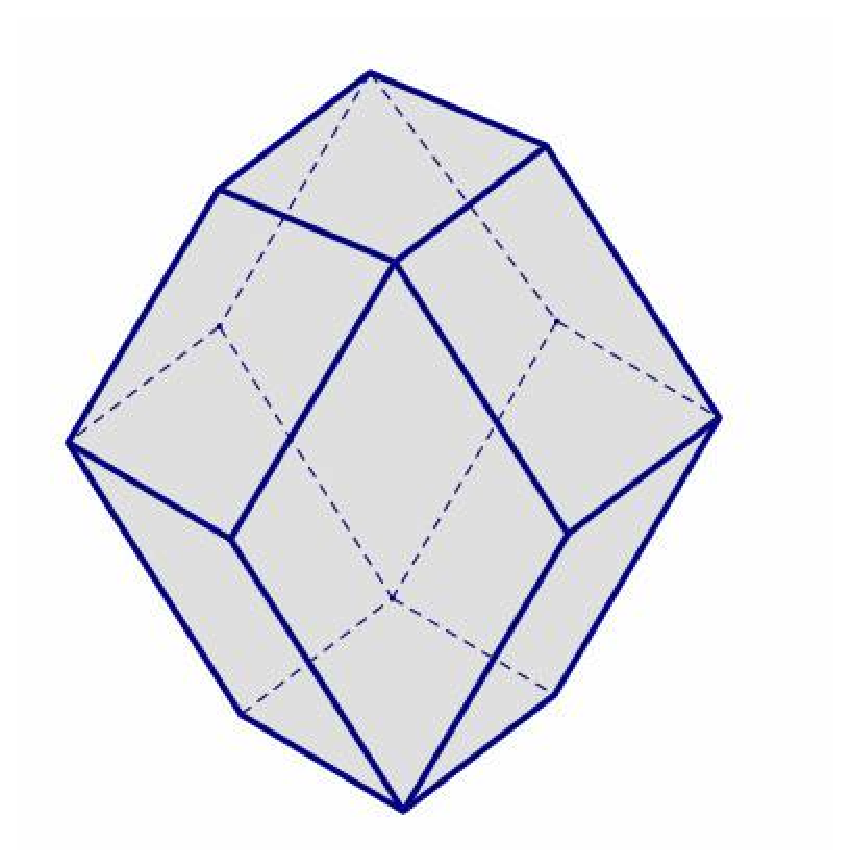
\includegraphics[width=5cm,height=4cm]{timg}
\end{frame}

% \begin{frame}
%   \frametitle{6.6 哈密顿图}
%   \centering
%   \vspace{-0.5cm}\uncover<2->{
%     \begin{tikzpicture}[auto,
%     specification/.style ={circle, draw, thick, inner sep = 0pt, minimum size=2mm}]
%    \node[specification] (A)  [label=-90:$v_1$] at (0,0)  {};
%    \node[specification] (B)  [label=-90:$v_2$] at (0.5,0)  {};
%    \node[specification] (C)  at (1,0)  {};
%    \node[specification] (D) at (1.5,0)  {};
%    \node[specification] (E)  [label=-90:$v_{i_{s-1}}$] at (2,0)  {};
%    \node[specification] (F)  [label=-90:$v_{i_s}$]at (2.5,0)  {};
%    \node[specification] (G)  at (3,0)  {};
%    \node[specification] (H)  at (3.5,0)  {};
%    \node[specification] (I) at (4,0)  {};
%    \node[specification] (J) [label=-90:$v_{k-1}$] at (4.5,0)  {};
%    \node[specification] (K) [label=-90:$v_k$] at (5,0)  {};
   
   
%    \draw[thick] (A) to  (B);
%    \draw[thick] (B) to  (C);
%    \draw[thick] (C) to  (D);
%    \draw[thick] (D) to  (E);
%    \draw[thick] (E) to  (F);
%    \draw[thick] (F) to  (G);
%    \draw[thick] (G) to  (H);
%    \draw[thick] (H) to  (I);
%    \draw[thick] (I) to  (J);
%    \draw[thick] (J) to  (K);
% %   \draw[thick] (A) to [bend left = 20] (F);
% %   \draw[thick] (K) to [bend left = 20] (E);
%  \end{tikzpicture}  }
%   \begin{Ex}
%     设$G$是一个有$p$个顶点$q$条边的图。证明:如果$p > 2\delta(G)$,则有长至少为$2\delta(G)$的路。
%   \end{Ex}\pause
%   \small{
%   \begin{proof}[证明]
%     设$G$中的最长路为$v_1v_2\cdots v_k$,\pause 只需证明$k \geq 2\delta(G) + 1$。\pause

%     用反证法,假设$k \leq 2\delta(G)$。 \pause 以下证明$v_1v_2\cdots v_k$必在同一个圈上。\pause
%     \begin{itemize}
%     \item 如果$v_1$与$v_k$邻接,则$v_1v_2\cdots v_kv_1$构成$G$中的一个圈;\pause
%     \item 如果$v_1$与$v_k$不邻接,由$v_1v_2\cdots v_k$为最长路知$v_1,v_k$只能与$v_2,v_3,\ldots,v_{k-1}$中的顶点邻接。
%     \end{itemize}

%   \renewcommand{\qedsymbol}{}    
%   \end{proof}}
% \end{frame}

% \begin{frame}
%   \frametitle{6.6 哈密顿图}
%   \centering
%   \vspace{-0.5cm}
%     \begin{tikzpicture}[auto,
%     specification/.style ={circle, draw, thick, inner sep = 0pt, minimum size=2mm}]
%    \node[specification] (A)  [label=-90:$v_1$] at (0,0)  {};
%    \node[specification] (B)  [label=-90:$v_2$] at (0.5,0)  {};
%    \node[specification] (C)  at (1,0)  {};
%    \node[specification] (D) at (1.5,0)  {};
%    \node[specification] (E)  [label=-90:$v_{i_{s-1}}$] at (2,0)  {};
%    \node[specification] (F)  [label=-90:$v_{i_s}$]at (2.5,0)  {};
%    \node[specification] (G)  at (3,0)  {};
%    \node[specification] (H)  at (3.5,0)  {};
%    \node[specification] (I) at (4,0)  {};
%    \node[specification] (J) [label=-90:$v_{k-1}$] at (4.5,0)  {};
%    \node[specification] (K) [label=-90:$v_k$] at (5,0)  {};
   
   
%    \draw[thick] (A) to  (B);
%    \draw[thick] (B) to  (C);
%    \draw[thick] (C) to  (D);
%    \draw[thick] (D) to  (E);
%    \draw[thick] (E) to  (F);
%    \draw[thick] (F) to  (G);
%    \draw[thick] (G) to  (H);
%    \draw[thick] (H) to  (I);
%    \draw[thick] (I) to  (J);
%    \draw[thick] (J) to  (K);
%    \draw[thick] (A) to [bend left = 20] (F);
%    \draw[thick] (K) to [bend left = 20] (E);
%  \end{tikzpicture}  
%   \begin{Ex}
%     设$G$是一个有$p$个顶点$q$条边的图。证明:如果$p > 2\delta(G)$,则有长至少为$2\delta(G)$的路。
%   \end{Ex}
%   \small{
%   \begin{proof}[证明]
%     设$G$中的最长路为$v_1v_2\cdots v_k$,只需证明$k \geq 2\delta(G) + 1$。

%     用反证法,假设$k \leq 2\delta(G)$。  以下证明$v_1v_2\cdots v_k$必在同一个圈上。
%     \begin{itemize}
%     \item 如果$v_1$与$v_k$邻接,则$v_1v_2\cdots v_kv_1$构成$G$中的一个圈;
%     \item 如果$v_1$与$v_k$不邻接,由$v_1v_2\cdots v_k$为最长路知$v_1,v_k$只能与$v_2,v_3,\ldots,v_{k-1}$中的顶点邻接。 设$v_{i_1},v_{i_2},\ldots,v_{i_r}$与$v_1$邻接,$2=i_1 < i_2 < \cdots < i_r < k$,则$v_k$必与某个$v_{i_s-1}$邻接,$2\leq s \leq r$。
%       否则,$v_k$至多与最长路上其余的顶点邻接,所以
%       \[\deg v_1 + \deg v_2 \leq r + ((k-1) - r) = k - 1 \leq 2\delta(G) - 1\]
%       矛盾。于是,$v_1v_2\cdots v_{i_{s-1}}v_kv_{k-1}\cdots v_{i_s}v_1$是$G$中的一个圈。总之,$v_1,v_2,\cdots,v_k$在$G$的同一个圈$C$上。
%     \end{itemize}

%   \renewcommand{\qedsymbol}{}    
%   \end{proof}}
% \end{frame}

% \begin{frame}[t]
%   \frametitle{6.6 哈密顿图}
%    \centering
%   \vspace{-0.5cm}
%     \begin{tikzpicture}[auto,
%     specification/.style ={circle, draw, thick, inner sep = 0pt, minimum size=2mm}]
%    \node[specification] (A)  [label=-90:$v_1$] at (0,0)  {};
%    \node[specification] (B)  [label=-90:$v_2$] at (0.5,0)  {};
%    \node[specification] (C)  at (1,0)  {};
%    \node[specification] (D) at (1.5,0)  {};
%    \node[specification] (E)  [label=-90:$v_{i_{s-1}}$] at (2,0)  {};
%    \node[specification] (F)  [label=-90:$v_{i_s}$]at (2.5,0)  {};
%    \node[specification] (G)  at (3,0)  {};
%    \node[specification] (H)  at (3.5,0)  {};
%    \node[specification] (I) at (4,0)  {};
%    \node[specification] (J) [label=-90:$v_{k-1}$] at (4.5,0)  {};
%    \node[specification] (K) [label=-90:$v_k$] at (5,0)  {};
   
   
%    \draw[thick] (A) to  (B);
%    \draw[thick] (B) to  (C);
%    \draw[thick] (C) to  (D);
%    \draw[thick] (D) to  (E);
%    \draw[thick] (E) to  (F);
%    \draw[thick] (F) to  (G);
%    \draw[thick] (G) to  (H);
%    \draw[thick] (H) to  (I);
%    \draw[thick] (I) to  (J);
%    \draw[thick] (J) to  (K);
%    \draw[thick] (A) to [bend left = 20] (F);
%    \draw[thick] (K) to [bend left = 20] (E);
%  \end{tikzpicture}  
%   \begin{proof}[证明(续上页)]
%     由于$G$是连通的,$p > 2\delta(G)$,所有$G$必有某个顶点$v$,$v$不在$C$上,但
%     与$C$上某个顶点$v_i$邻接。于是得到$G$的一条更长的路,这就出现了矛盾。
    
%   \end{proof}
% \end{frame}
\section{图的邻接矩阵}
% \begin{frame}
%   \frametitle{6.7 图的邻接矩阵}
% \centering
% \includegraphics[width=5cm,height=4cm]{representation} 
% \end{frame}

\begin{frame}
  \frametitle{6.7 图的邻接矩阵}
  \begin{Thm}
    设$G=(V,E)$为一个(p,q)图,$p\times p$矩阵$A$为$G$的邻接矩阵,则$G$中$v_i$与
    $v_j$间长为$l$的通道的条数等于$A^l$的第$i$行第$j$列元素的值。
  \end{Thm}
    \centering
  \begin{tikzpicture}[auto,
    specification/.style ={circle, draw, thick}]
   \node[specification] (E) [label=-135:$v_5$] at (0,0)  {};
   \node[specification] (F) [label=135:$v_3$] at (0,2)  {};
   \node[specification] (G) [label=45:$v_2$] at (2,2)  {};
   \node[specification] (H) [label=-45:$v_4$] at (2,0)  {};
   \node[specification] (I) [label=-45:$v_1$] at (4,2)  {};
   
   \draw[thick] (E) to  (F);
   \draw[thick] (F) to  (G);
   \draw[thick] (G) to  (H);
   \draw[thick] (H) to  (E);
   \draw[thick] (E) to  (G);
   \draw[thick] (G) to  (I);
 \end{tikzpicture}  
 \\  G   
\end{frame}



% \begin{frame}
%   \frametitle{6.8 带权图与最短路问题}

% \end{frame}

\end{CJK*}
\end{document}

%%% Local Variables:
%%% mode: latex
%%% TeX-master: t
%%% End:
